\chapter{Installation}
In diesem Kapitel gehen wir auf die Installation der Simplifizierung ein. Da
dieses Projekt auch in zukünftigen Projekten verwendet werden soll muss eine
Installationsbeschreibung vorhanden sein. Diese soll dem Administrator eine
einfache Installation ermöglichen.\\
Die Installation sollte nur von einem Administrator durchgeführt werden. 
Die zu installierenden Dateien sind in einem zip bzw. rar Archiv verpackt. 
Natürlich wird eine ordentliche Installation von Rhapsody vorausgesetzt. Der
Rest lässt sich grob Grob in drei Punkte aufteilen.
Dazu gehören:
\begin{itemize}
  \item Installation von Eclipse (Optional)
  \item Anpassen der hep Datei bzw. rein kopieren (Benutzerdoku)
  \item Projekte installieren bzw. erzeugen
\end{itemize}
Der Installationsort für Eclipse und die Version ist hierbei egal. Eigentlich
wird Eclipse nur benötigt um die User-Simplifizierung zu bauen. Die benötigten
Dateien legt Eclipse standardmäßig in einem "bin" Ordner ab. Dieser Ordner ist
wichtig. Aus diesem Ordner werden die Dateien gelesen und Rhapsody erstellt
unsere Pattern. Bei unseren Projekten befindet sich das Rhapsody-Projekt im
Eclipse Workspace. Dies ist jedoch nicht erforderlich. 
\begin{figure}[H]
	\centering
	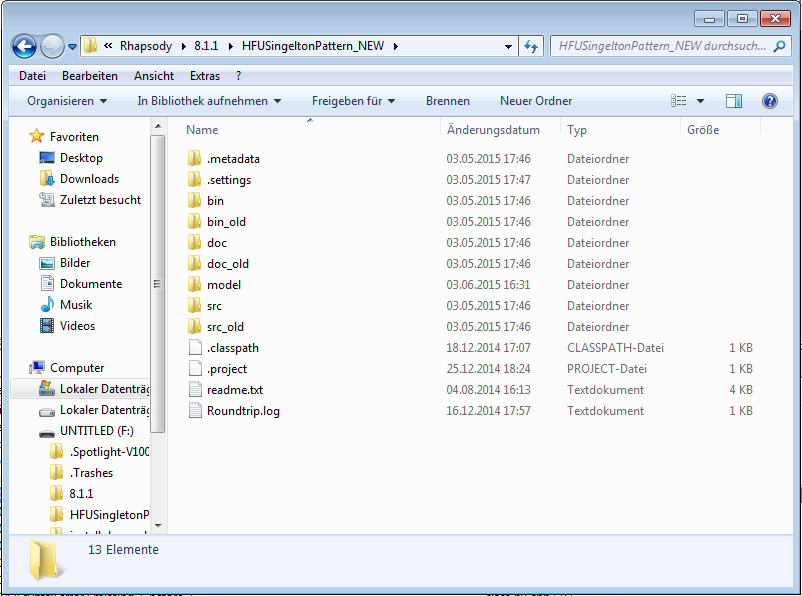
\includegraphics[width=0.79\textwidth]{content/pictures/install/struktur.png}
	\label{pic:bild}
	\caption{Ordnerstruktur von Eclipse-Workspace}
\end{figure}
Im Ordner model befindet sich das jeweilige Rhapsody-Projekt. Dies ist nur für
Tests sinnvoll. Bei der normalen Entwicklung darf der User seine Projekte in
einem beliebigen Verzeichnis ablegen. Damit Rhapsody jetzt auch weiß das wir
eine User-Simplifizierung haben, muss die hep Datei angepasst werden. Diese befindet sich im model-Ordner und in dem jeweiligen angelegten
Projekt mit der Endung _rpy.
\begin{figure}[H]
	\centering
	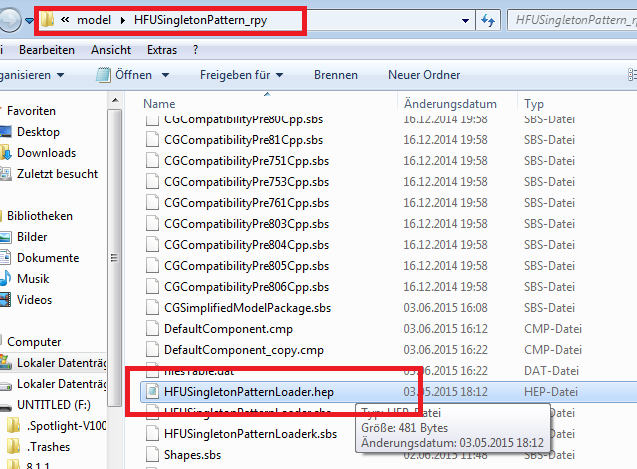
\includegraphics[width=0.88\textwidth]{content/pictures/install/model.png}
	\label{pic:bild}
	\caption{Erstelltes Projektverzeichniss}
\end{figure}
Die .hep Datei kann mit einem Texteditor geöffnet werden und angepasst werden.
In unserem Fall sieht diese folgendermaßen aus.
\begin{figure}[H]
	\centering
	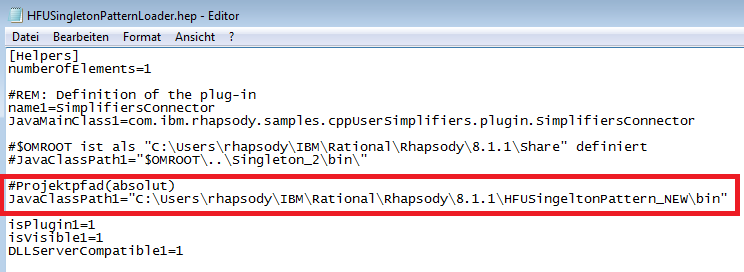
\includegraphics[width=0.8\textwidth]{content/pictures/install/hep.png}
	\label{pic:bild}
	\caption{Hep Datei}
\end{figure}
Hierbei interessiert uns nur die rote Markierung. Hier sieht man auch den
anfangs erwähnten bin Ordner. Ziel ist es eigentlich alle implementierten
Design-Pattern in einem Projekt zu Verfügung zu stellen.\\
Da aber auch in zukünftigen Projekten auf diese User-Simplifizierung zugegriffen
werden soll, ist es sinnvoll auch Eclipse zu installieren. Hier kann dann ganz
einfach die Simplifizierung angepasst werden. Da es hier keine main-Funktion
gibt, gibt es auch keinen ausführbaren Code. Eclipse erstellt durch das
Speichern der Dateien die .class Dateien, die wiederum im bin Ordner des
Projekts landen.\\ 
\textbf{WICHTIG}\\
Fals die Implementierung angepasst bzw. geändert wird, muss
Rhapsody beendet werden und erneut gestartet werden. Erst jetzt ist die Änderung
wirksam.  
\begin{figure}[H]
	\centering
	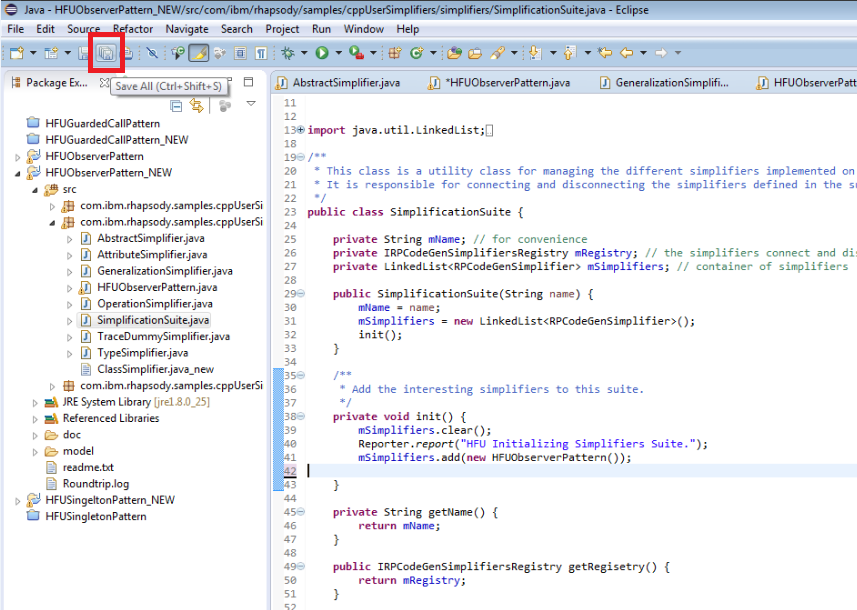
\includegraphics[width=0.88\textwidth]{content/pictures/install/saveBin.png}
	\label{pic:bild}
	\caption{Speichern und Erstellen der .class Dateien}
\end{figure}




